\subsubsection{Карта рассеяния в обратном пространстве}

\begin{figure}[H]
  \centering
  \subfloat[Точное бреговское положение]{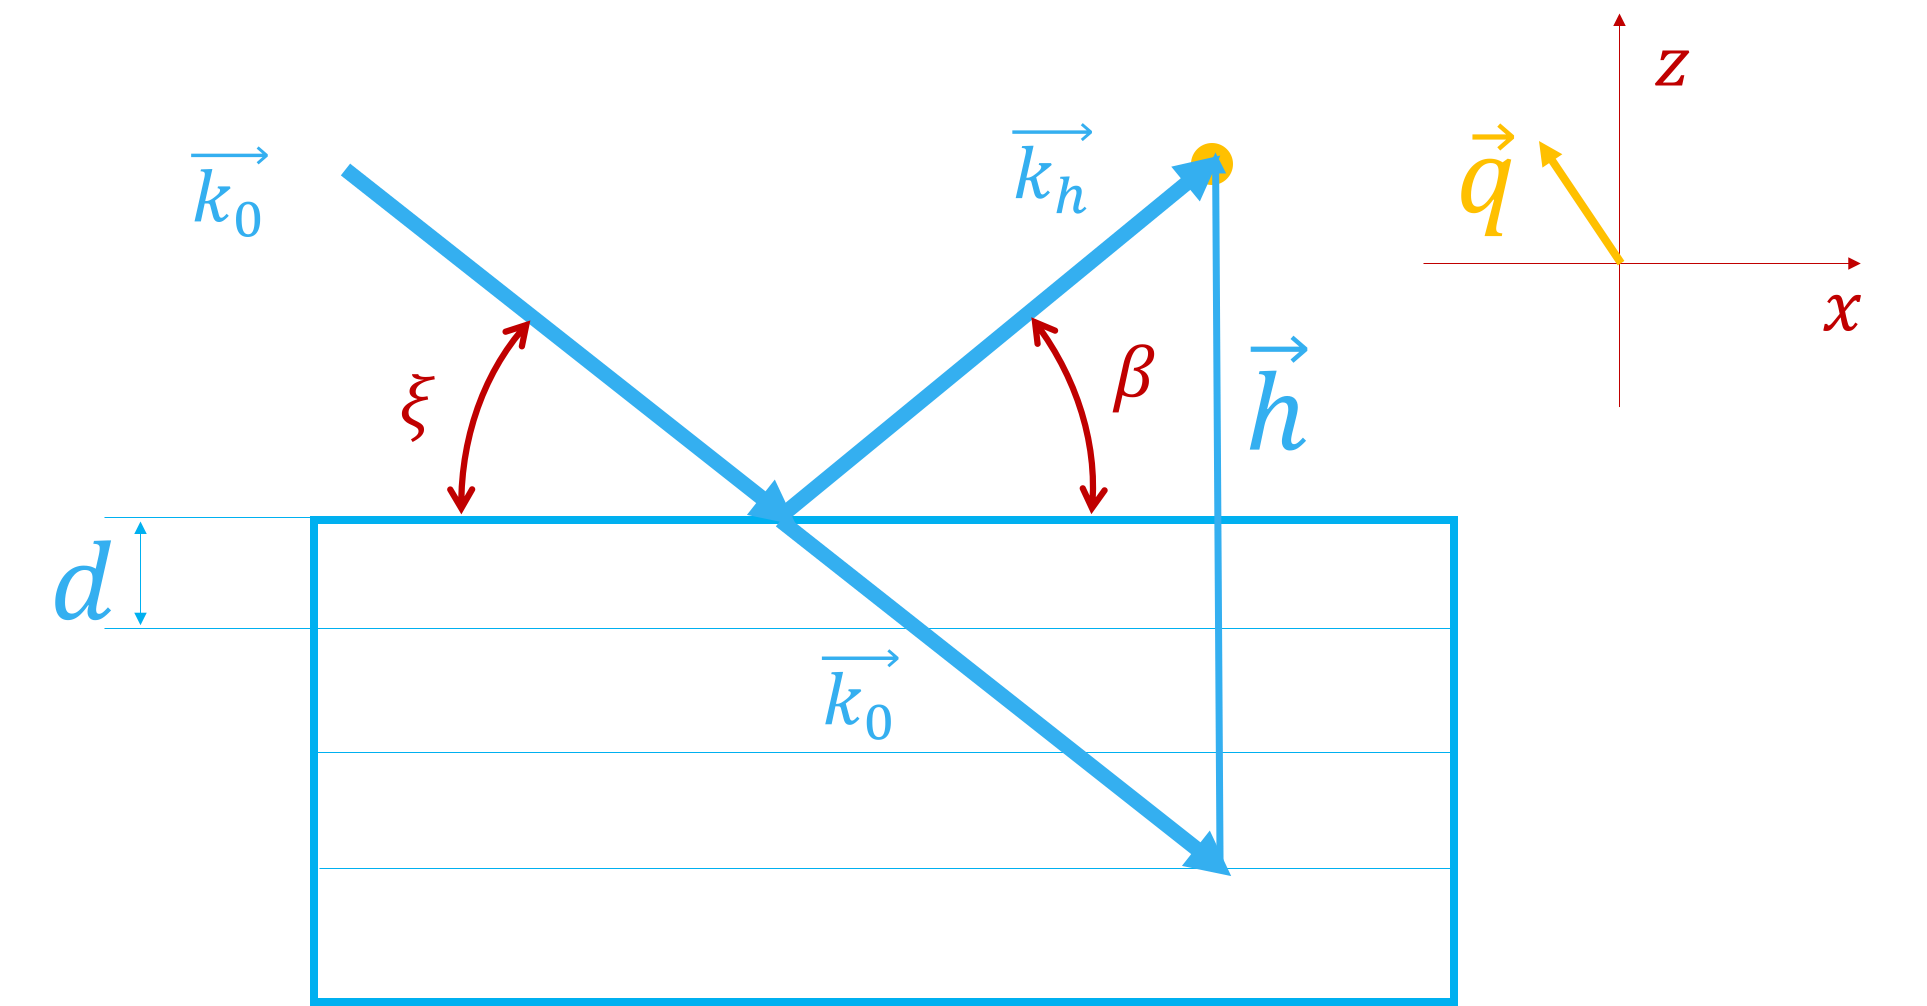
\includegraphics[width=0.3\textwidth]{images/q_vector/0.png}}
  \hfill
  \subfloat[Около брегговское положение - деформация]{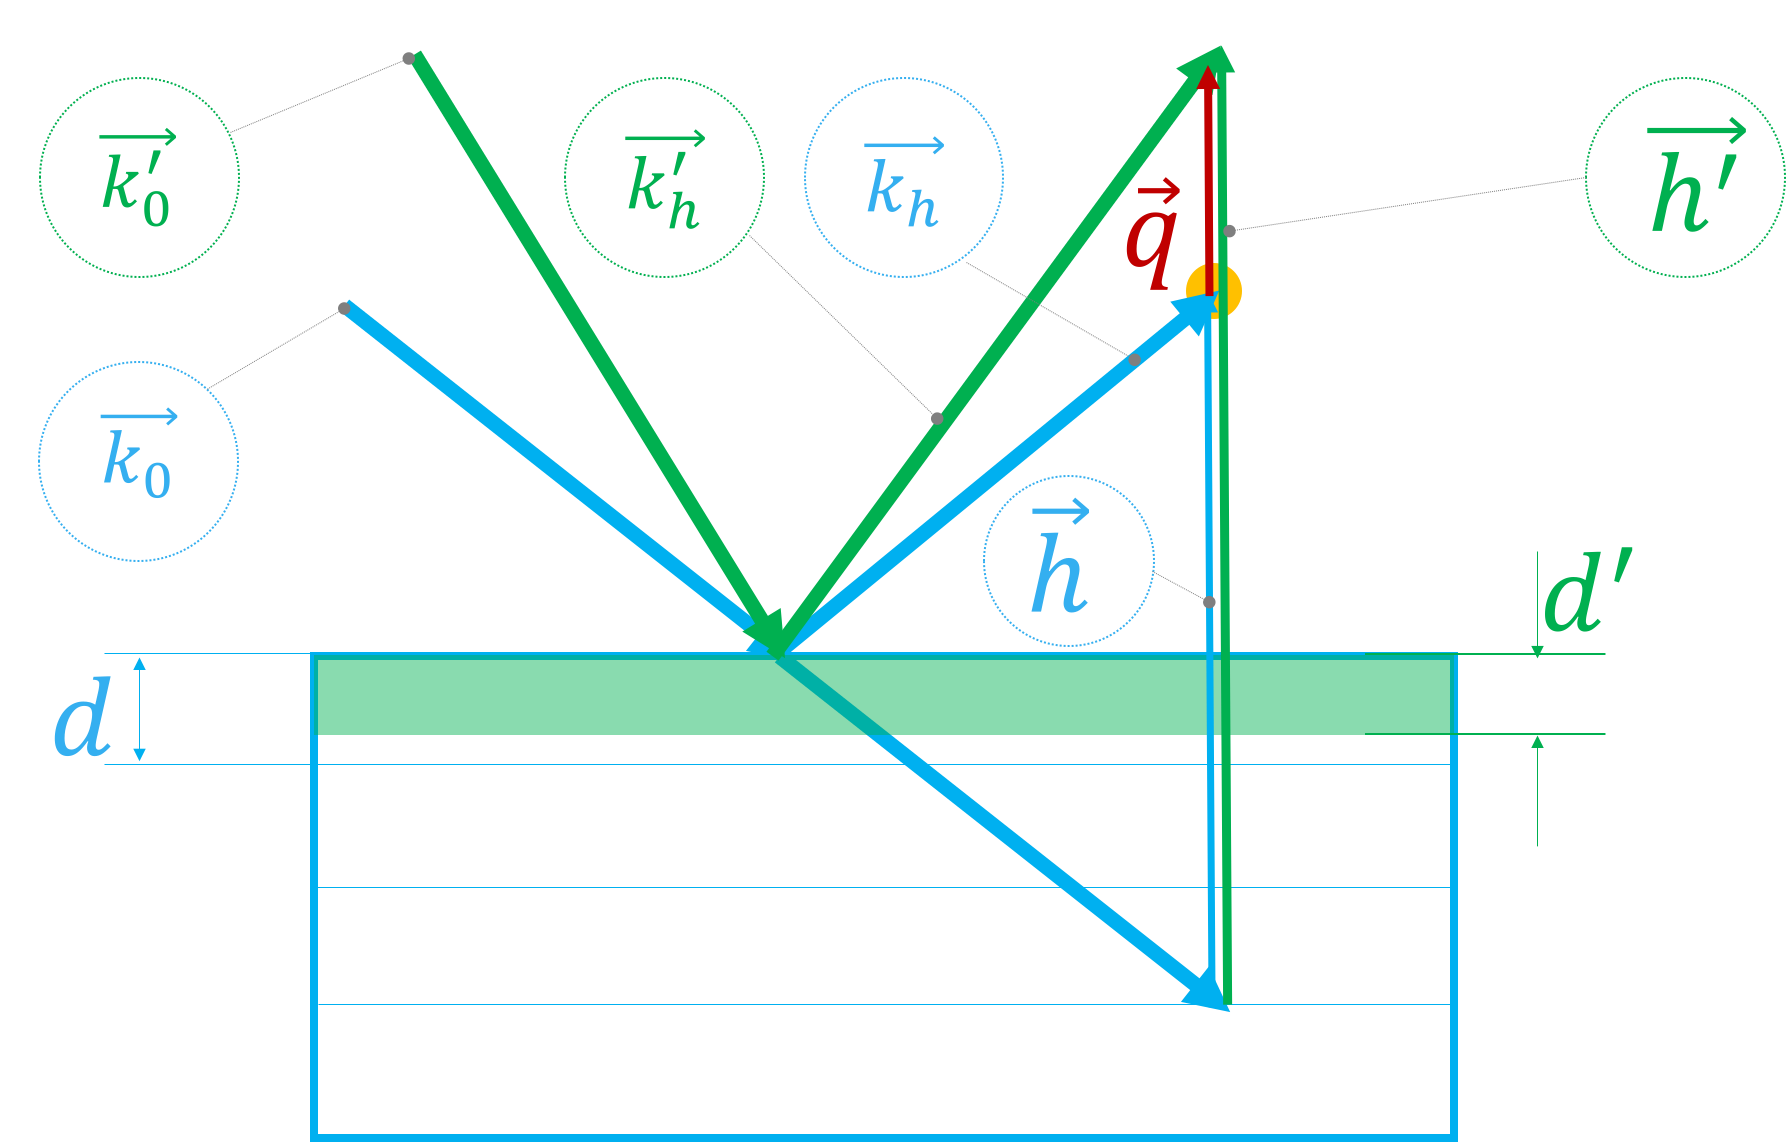
\includegraphics[width=0.3\textwidth]{images/q_vector/_1.png}}
  \hfill
  \subfloat[Около брегговское положение - разориентация]{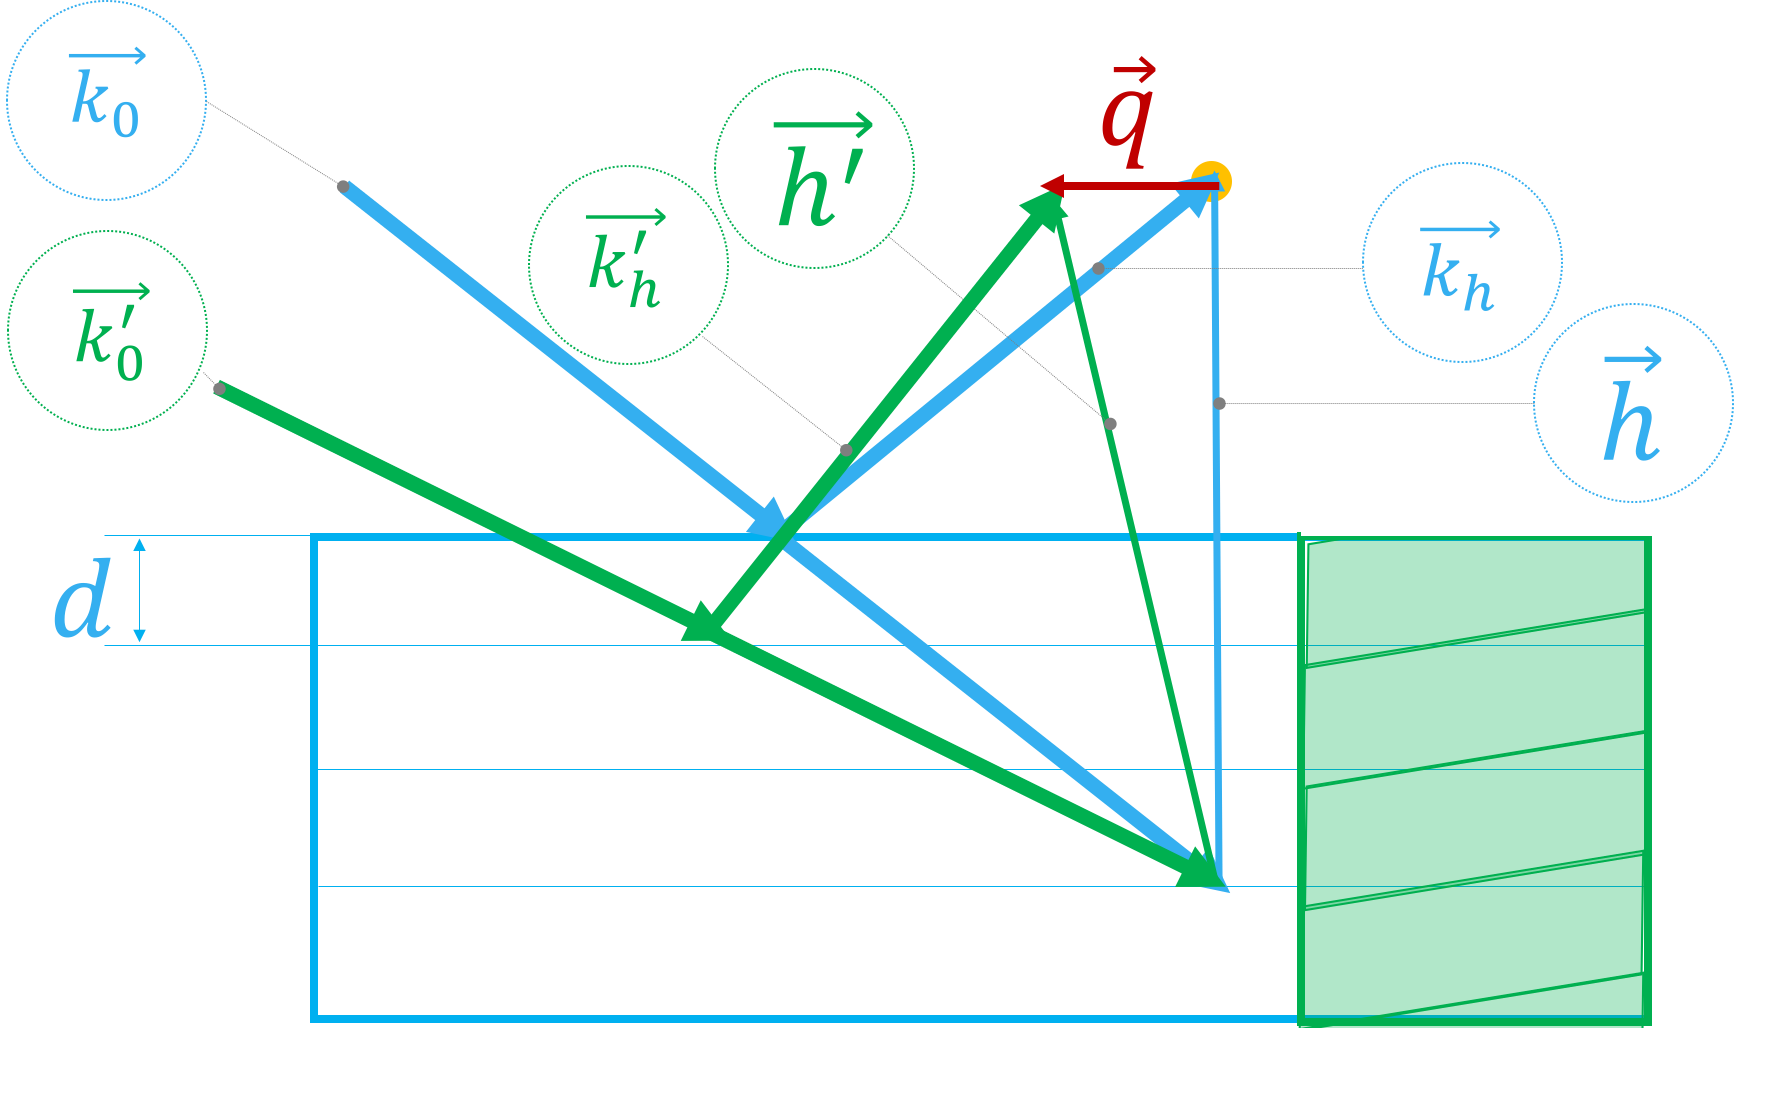
\includegraphics[width=0.3\textwidth]{images/q_vector/1.png}}
  \caption{Отклонение вектора обратной решетки от точного положения}
  \label{ris:}
\end{figure}



Вывод пересчетных формул в случае симмитричного случая отражения представлен в ()


\cite{Tanner_1998}
